\documentclass[crop,tikz]{standalone}

\usepackage{amsmath}
\tikzset{>=latex}
\usetikzlibrary{calc,patterns}
\newcommand{\F}{\vec{F}}
\newcommand{\ort}{\vec{r}}
\newcommand{\vs}{\vec{s}}

\begin{document}
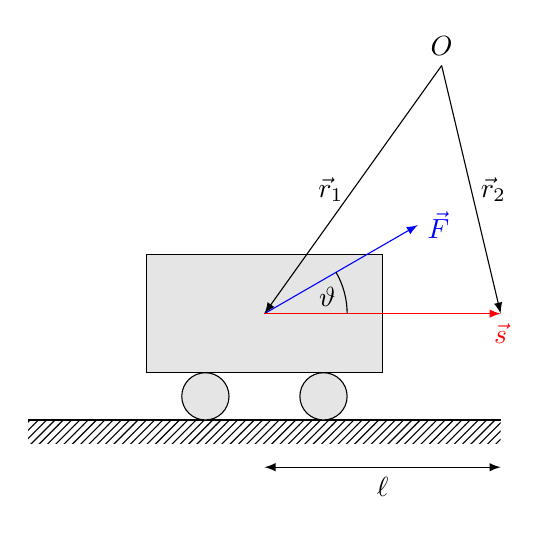
\begin{tikzpicture}[scale=1.5]
  \pgfmathsetmacro{\angl}{30}
  \pgfmathsetmacro{\wheel}{0.2}
  \pattern[pattern=north east lines] (-1,0)--++(0,-0.2)--++(4,0)--++(0,0.2)--cycle;
  \draw (-1,0) -- ++(4,0);
  \draw[fill=gray!20] (0.5,\wheel) circle (\wheel);
  \draw[fill=gray!20] (1.5,\wheel) circle (\wheel);
  \draw[fill=gray!20] (0,2*\wheel) rectangle (2,1+2*\wheel);
  \coordinate (C) at (1,2*\wheel+0.5);
  \coordinate (Z) at (3,2*\wheel+0.5);
  \draw[->,blue] (C) -- ++(\angl:1.5) node[right] {$\F$};
  \draw[->,red]  (C) -- (Z) node[below] {$\vs$};
  \draw (C)+(0:0.7) arc (0:\angl:0.7);
  \node at ($(C)+({\angl/2}:0.55)$) {$\vartheta$};
  \draw[<->] (1,-0.4) -- node[below] {$\ell$} +(2,0);
  \coordinate (O) at (2.5,3);
  \node[above] at (O) {$O$};
  \draw[->] (O) -- node[left] {$\ort_1$} (C);
  \draw[->] (O) -- node[right] {$\ort_2$} (Z);
\end{tikzpicture}
\end{document}
